\subsection{Scalar Fields > Filter by Value}
\label{subsection:scalarFieldFilterByValue}

\begin{figure}[!htb]
\begin{center}
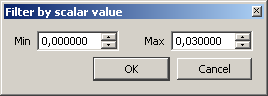
\includegraphics[width=0.32\textwidth]{Partie3_Fonctions/sfFilterByValueDlg.png}
\caption{\label{fig:sfFilterByValueDlg}Interface de param�trage pour le filtrage des points selon la valeur du champ scalaire actif}
\end{center}
\end{figure}

\index{champ scalaire}
\index{segmentation}
Cette fonction permet de segmenter un nuage en d�finissant un intervalle de valeurs scalaires (figure~\ref{fig:sfFilterByValueDlg}). Un nouveau nuage sera cr�� avec tous les points dont les valeurs scalaires (tir�es du champ scalaire actif) sont inclues dans cet intervalle. Lors de l'appel de la fonction, les valeurs par d�faut de la boite de dialogue correspondent aux valeurs \textit{min displayed} et \textit{max displayed} des param�tres d'affichage du champ scalaire actif (voir section~\ref{Champs-scalaires}).
